\section{Compound DMA attacks}\label{sec:linux_net}

%\adam{This section is significantly less organized than the rest of the paper (the fact you discuss IOTLB in two places is an example. I suggest to organize it according to the characterizations: first explain how the networking system design makes the 3/4 vulnerability types occur, then have sections according to the trifecta where you explain how those are obtained, and title them accordingly, not with cute but not meaningful names. Following my comment about the 3rd ``sub-page'' vuln type (multiple mapping), which doesn't belong as a vuln type, I suggest introducing that here (since really, this is what's happening anyway).}

%\adam{I'd retitle this section: it is about kernel design flaws to enable getting Motive, Means, and Opportunity}

%So far, we have demonstrated a \simple attack by exploiting type (a) \subpage vulnerability of the FireWire driver. 
This section explores new attacks on the Linux network stack where the vulnerability attributes are initially missing but are attainable via compound steps.
We focus on the Linux network stack which initially seems secure~\cite{thunder}.
Nevertheless, as we demonstrate, the Linux network stack is actually responsible for 60\% of \textcolor{red}{the} DMA vulnerabilities we have found.

Recall that, once we have discovered a \subpage{} vulnerability, our goal is to obtain the three vulnerability attributes (Sec. \ref{sec:mmo}: (1) a KVA, (2) a callback pointer and, (3) timing). 
Accordingly, in Sec.~\ref{sec:shinfo_exploit}, we first describe how to obtain (2) a callback function pointer. Then, in Sec.~\ref{sec:timely}, we show that (3) a time window for exploiting this pointer is available. 
While these two steps for obtaining vulnerability attributes (2) and (3) are generic, there are different recipes for how to obtain the remaining vulnerability attribute (1), i.e., the KVA of the malicious buffer. \sout{exposes via the \subpage{} vulnerability.}
We complete the vulnerability attributes in Sec.~\ref{sec:ringflod} and Sec.~\ref{sec:posion} by showing different ways (by which we also name the compound attack) to obtain (1) the KVA.



Due to space limitations we demonstrate only selected compound DMA attacks. 
Upon the publication of our work, we aim to release extended material, including evaluation scripts and additional \compound and previously unknown \simple attacks found by our tools.
%\sout{We first describe the vulnerable data structures shared by \emph{all} Linux network drivers, which exposes a callback pointer. Then, after providing some necessary technical background (Sec.~\ref{sec:deferred}), we show how that the device is often provided with a timing window during which a modified callback pointer will be executed by the CPU~(Sec.~\ref{sec:shinfo}). Finally, we discuss various methods to identify kernel virtual addresses of pages containing malicious code (Sec.~\ref{sec:ringflod} and~\ref{sec:posion}).}
%In the interest of space, additional methods for gaining \motivation are deferred to Appendix~\ref{appx:additional_compound}.

\subsection{Obtaining a callback pointer}\label{sec:shinfo_exploit}
\begin{figure}[t]
    \centering
    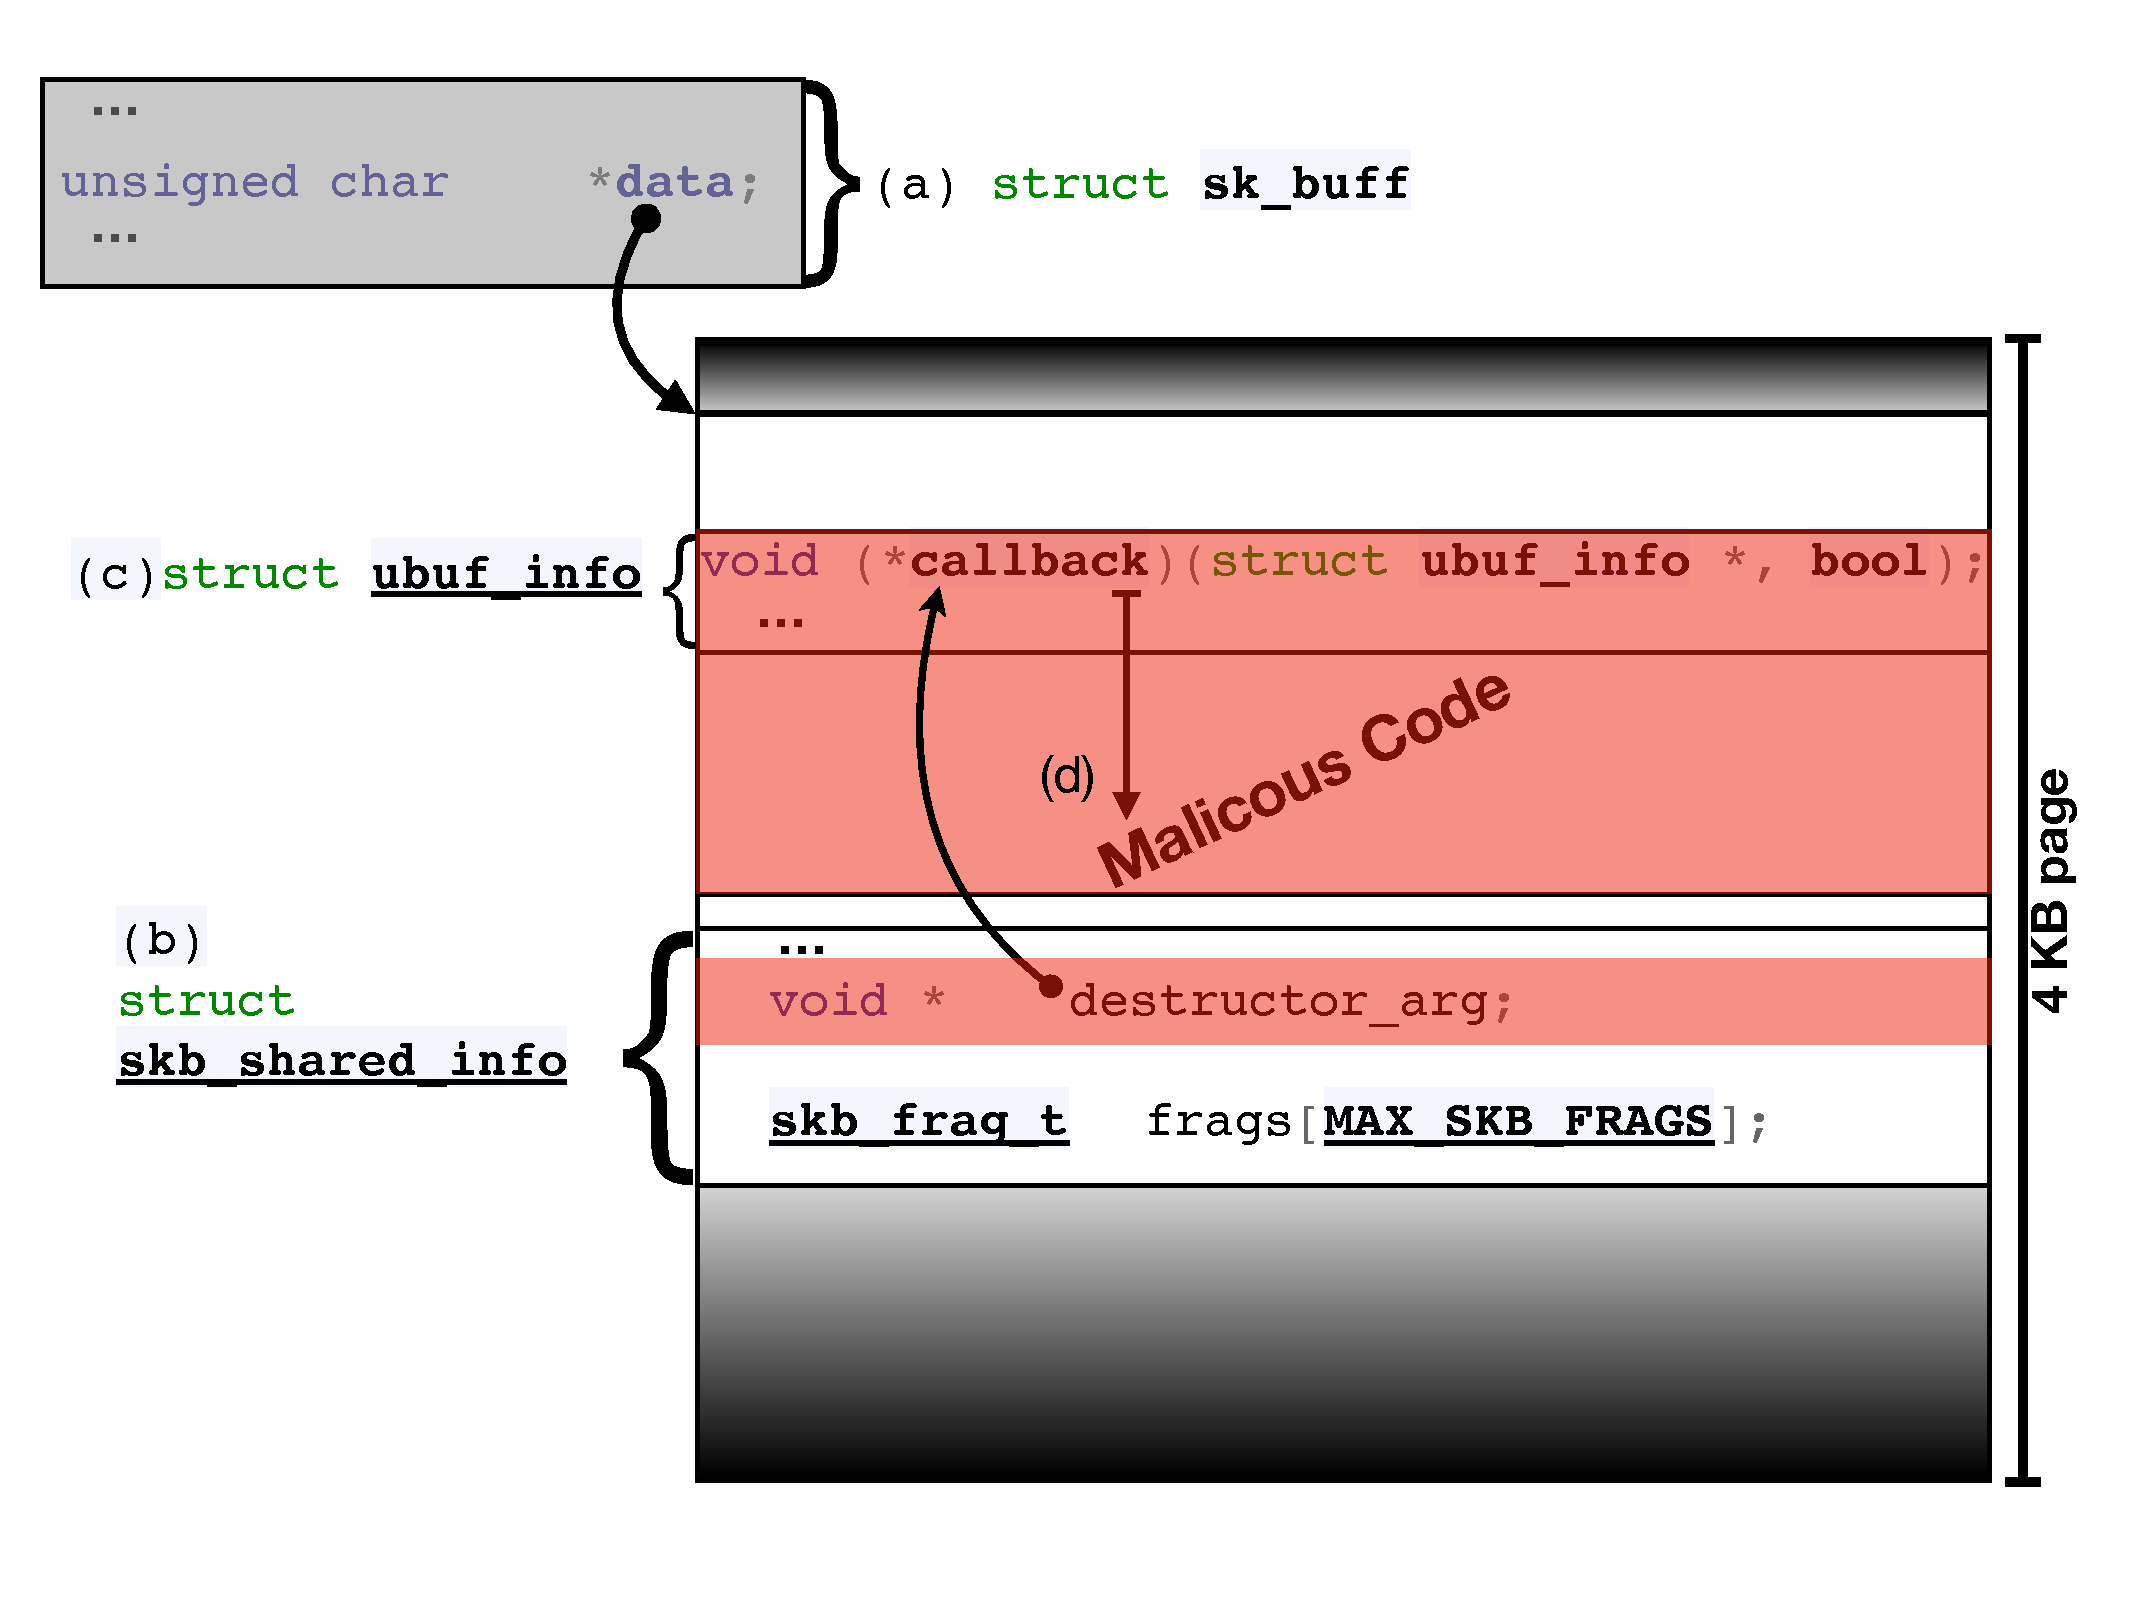
\includegraphics[width=0.8\linewidth]{figs/ubuf.pdf}
    \caption{Using \shinfo{} to execute arbitrary code in kernel context.}
    \label{fig:sh_info}
    %\vspace{-4mm}
\end{figure}

%\adam{lots of explanations here, whereas the structure was originally mentioned when talking about SCAT...}
Struct \skb{} is a data structure used by the Linux network stack to hold information representing a network packet. Struct \skb{} holds the metadata of a network packet (e.g., packet size, associated socket). One of these fields is a pointer to a data buffer. The data is allocated separately, and thus, does not share a page with its \skb{} (Fig.~\ref{fig:sh_info}). 

This separation means that \skb{} is \emph{never} (intentionally) mapped to the device. Indeed, it is a common belief\sout{, pointed out in the literature}\textcolor{red}{~(e.g., Markettos et al.~\cite{thunder})}, that the Linux network stack is not susceptible to DMA attacks via the \texttt{data} pointer. In this work, we show that this belief is misplaced.

The Linux network stack supports packet cloning by merely copying \skb{} metadata. \sout{This includes the \texttt{data} pointer.} That is, the resulting \skb{} and the original one share the \texttt{data} buffer~\cite{drivers2005linux}. \sout{Note that the \texttt{data} buffer of the \skb{} is the \emph{linear} part of the payload but \skb{} also supports \emph{non-linear} buffers.}\textcolor{red}{The payload in the \skb{} can be partially located on the \emph{liner} part~(i.e., in the buffer indicated by the \texttt{data} pointer) and partially on the \emph{non-linear} fragments.} That is, buffers that are described by their \page{}, length and offset in the \texttt{frags} array of \shinfo{} (Fig.~\ref{fig:sh_info}). 

To support the sharing of these non-linear buffers, the embedded \shinfo{} metadata structure is used.
Struct \shinfo{}, in contrast to \skb{}, is \emph{always} allocated as part of the data buffer. Therefore it is \emph{always} mapped to the device. \shinfo{} is unwittingly mapped with the permissions of the packet, i.e., WRITE for RX packets, READ for TX packets, and in some cases, such as XDP~\cite{xdp} with BIDIRECTIONAL.

Consequentially, \shinfo{} holds the potential callback pointer that the malicious device can exploit.\textcolor{red}{The \texttt{destructor\_arg} is used for socket buffer accounting and facilitates custom handling when the buffer is freed.} The \subpage{} vulnerability created by \shinfo{}, represents a type (b) vulnerability (Fig.~\ref{fig:colocation} (b)), as this is innate to Linux networking rather than a driver security bug. 

Fig.~\ref{fig:sh_info} depicts how a malicious device can mount an attack using \shinfo{} in four steps:
\begin{enumerate}[label=(\alph*)]
    \item An RX \skb{} and its data buffer are allocated. The data buffer is mapped for the NIC with WRITE access (the WRITE access is to the whole 4~KB page). 
    \item The NIC overwrites the \texttt{destructor\_arg} field in \shinfo{} to point within the mapped page. As a result, the \texttt{destructor\_arg} points to a struct \uarg{} which is created by the NIC.
    \item \uarg{} has a callback pointer that is now pointing to the malicious code residing on the same page. In the case of NX-bit, it is a poisoned ROP/JOP\cite{BJFL11} stack (Sec.~\ref{sec:nx-bit}).
    %\adam{how does this work? you overwrite a pointer to a callback function, not to the stack pointer.}\SV{a JOP attack, aslo mentioned in 2.4}
    \item when the \skb{} is released, the callback is invoked.
\end{enumerate}
To expand this scenario into a complete attack, the attacker must obtain all three vulnerability attributes. That is, the attacker needs the actual \kva{} of the \mabaf{} and the NIC must have a timely WRITE access to the page. In the next subsection, we demonstrate how an attacker can leverage standard OS behavior to obtain both missing vulnerability attributes.

\begin{figure}[t]
    \centering
    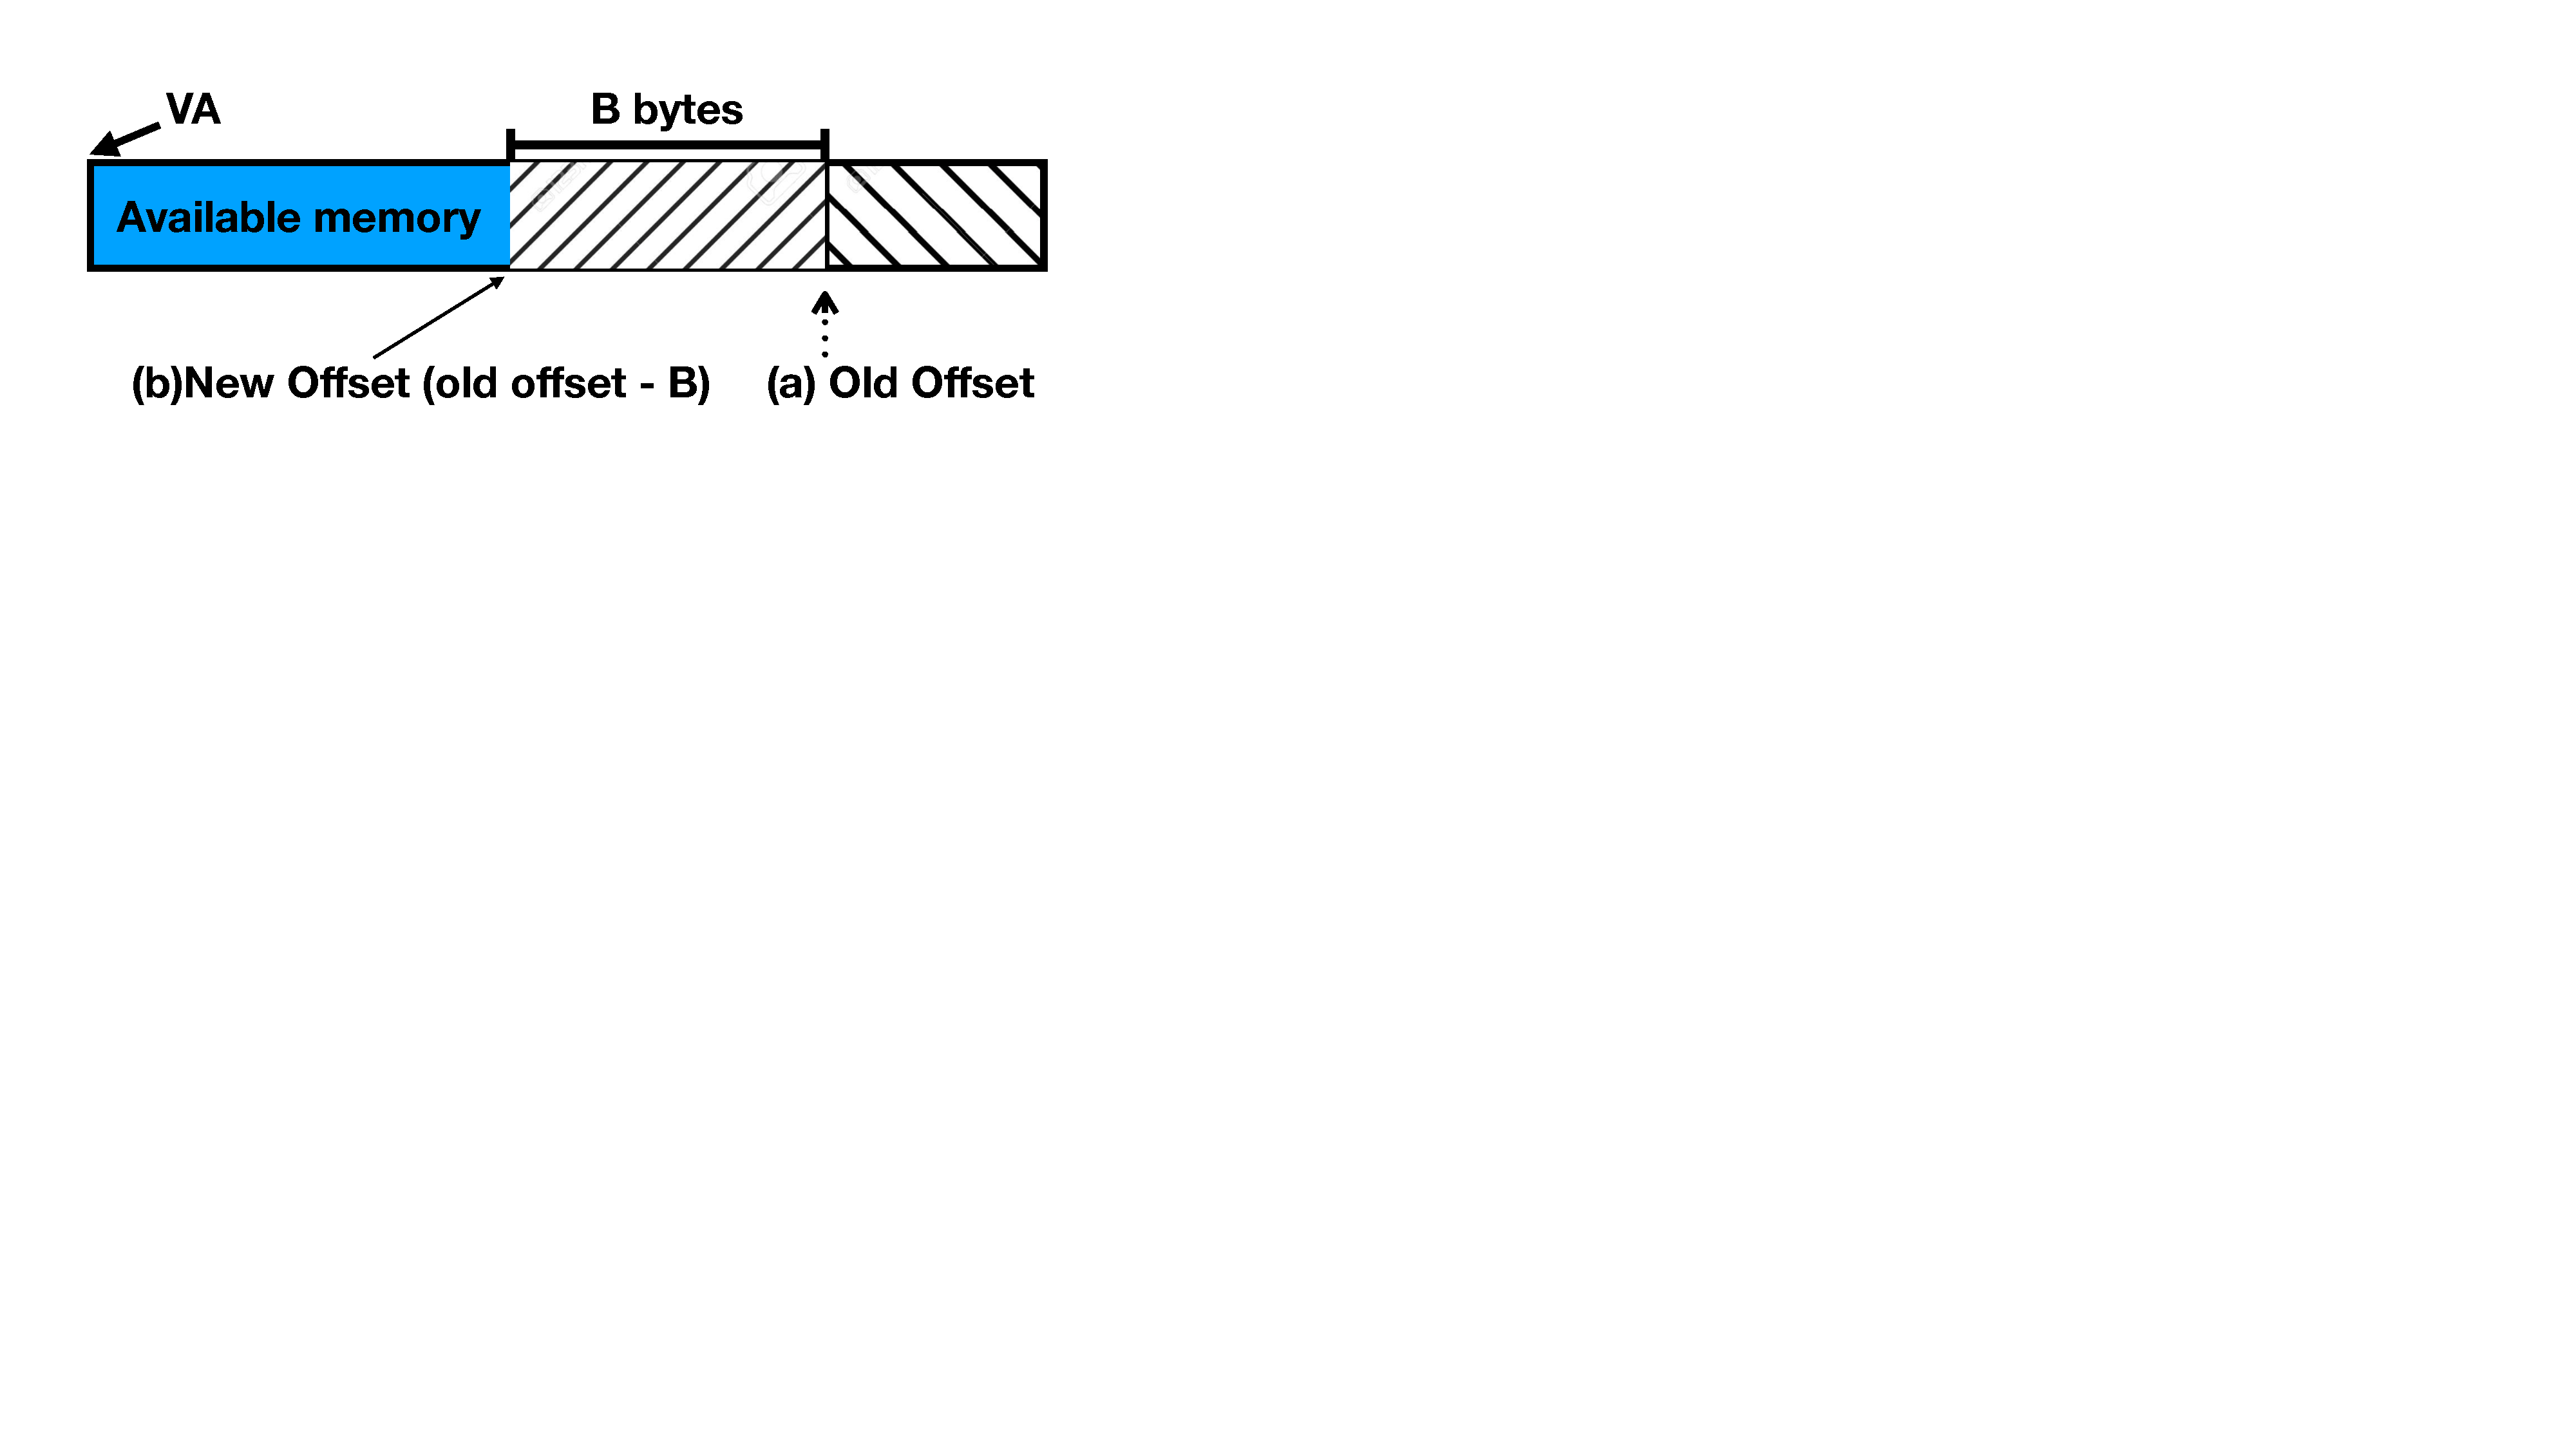
\includegraphics[width=0.65\linewidth,trim=0 6cm 0 6cm, clip]{figs/page_frag.pdf}
    \caption{Allocation of B bytes from page\_frag}
    \label{fig:page_frags}
\end{figure}

\subsection{Existence of a Time Window}\label{sec:timely}
To reason about the existence of an appropriate time window for altering the callback pointer, we first discuss the Linux default mode for IOTLB invalidation, which is a known security vulnerability~\cite{MMT16,MSMT18}.
In particular, in Sec.~\ref{sec:deferred} we present the issue of deferred invalidation. Then, in Sec.~\ref{sec:shinfo} we discuss the multiple means by which an attacker can gain timely access to \shinfo.

\subsubsection{Deferred Invalidation Vulnerability}\label{sec:deferred}
The IOTLB is analogous to the MMU TLB. The IOMMU does not maintain consistency between the IOTLB and the IOMMU page tables. As a result, the OS has to explicitly invalidate the IOTLB to maintain consistency when a translation entry is removed. Namely, to ensure that the IOTLB never holds stale entries, the OS must invalidate the IOTLB entry immediately after removing a DMA mapping. 

This scheme, called \emph{strict} mode in Linux, can degrade performance due to the overhead of IOTLB invalidations following each I/O operation ~\cite{MMT16,MSMT18,Peleg15}. In I/O intensive workloads, the combined cost of IOTLB invalidations can be prohibitively high. The overhead of each IOTLB invalidation can be as high as 2000 cycles~\cite{ABYTS11}. This overhead is considerably higher than a TLB invalidation, which takes roughly 100 cycles~\cite{Han14}. 

To reduce this overhead, Linux uses deferred mode as a default. Linux defers specific IOTLB invalidations and instead performs periodic global IOTLB invalidations. While this \emph{deferred} mode improves I/O performance, it also breaks the stipulation that after unmapping (e.g., \texttt{dma\_unmap\_page}), the physical page should no longer be accessible by the device. This \emph{deferred} time frame (Fig.~\ref{fig:deferred}) may be as high as 10 milliseconds~\cite{MSMT18}.

The repercussions of \emph{deferred} mode are that a malicious device can take advantage of this time window, where it has access to memory pages unbeknownst to the CPU. \emph{deferred} mode opens up two distinct attack options:

\begin{enumerate}[labelindent=0pt]
    \item A device can alter data structures that the CPU has modified \emph{after} unmapping (e.g., calling \texttt{dma\_unmap\_page}).
    \iova{} mappings, as a rule, are short-lived as they should be used only for the duration of I/O, usually for a few microseconds. The additional milliseconds provide the attacker with a wide time window sufficient to conduct its attack.
    \item The page can be freed and then immediately reused by the OS. Fast reuse is a common scenario since Linux reuses \emph{hot} pages (i.e., recently used pages) as they are likely to reside in the CPU caches~\cite{hotcold}. However, this also opens up the kernel to additional random access attacks.
\end{enumerate}



\begin{figure}[t]
    \centering
    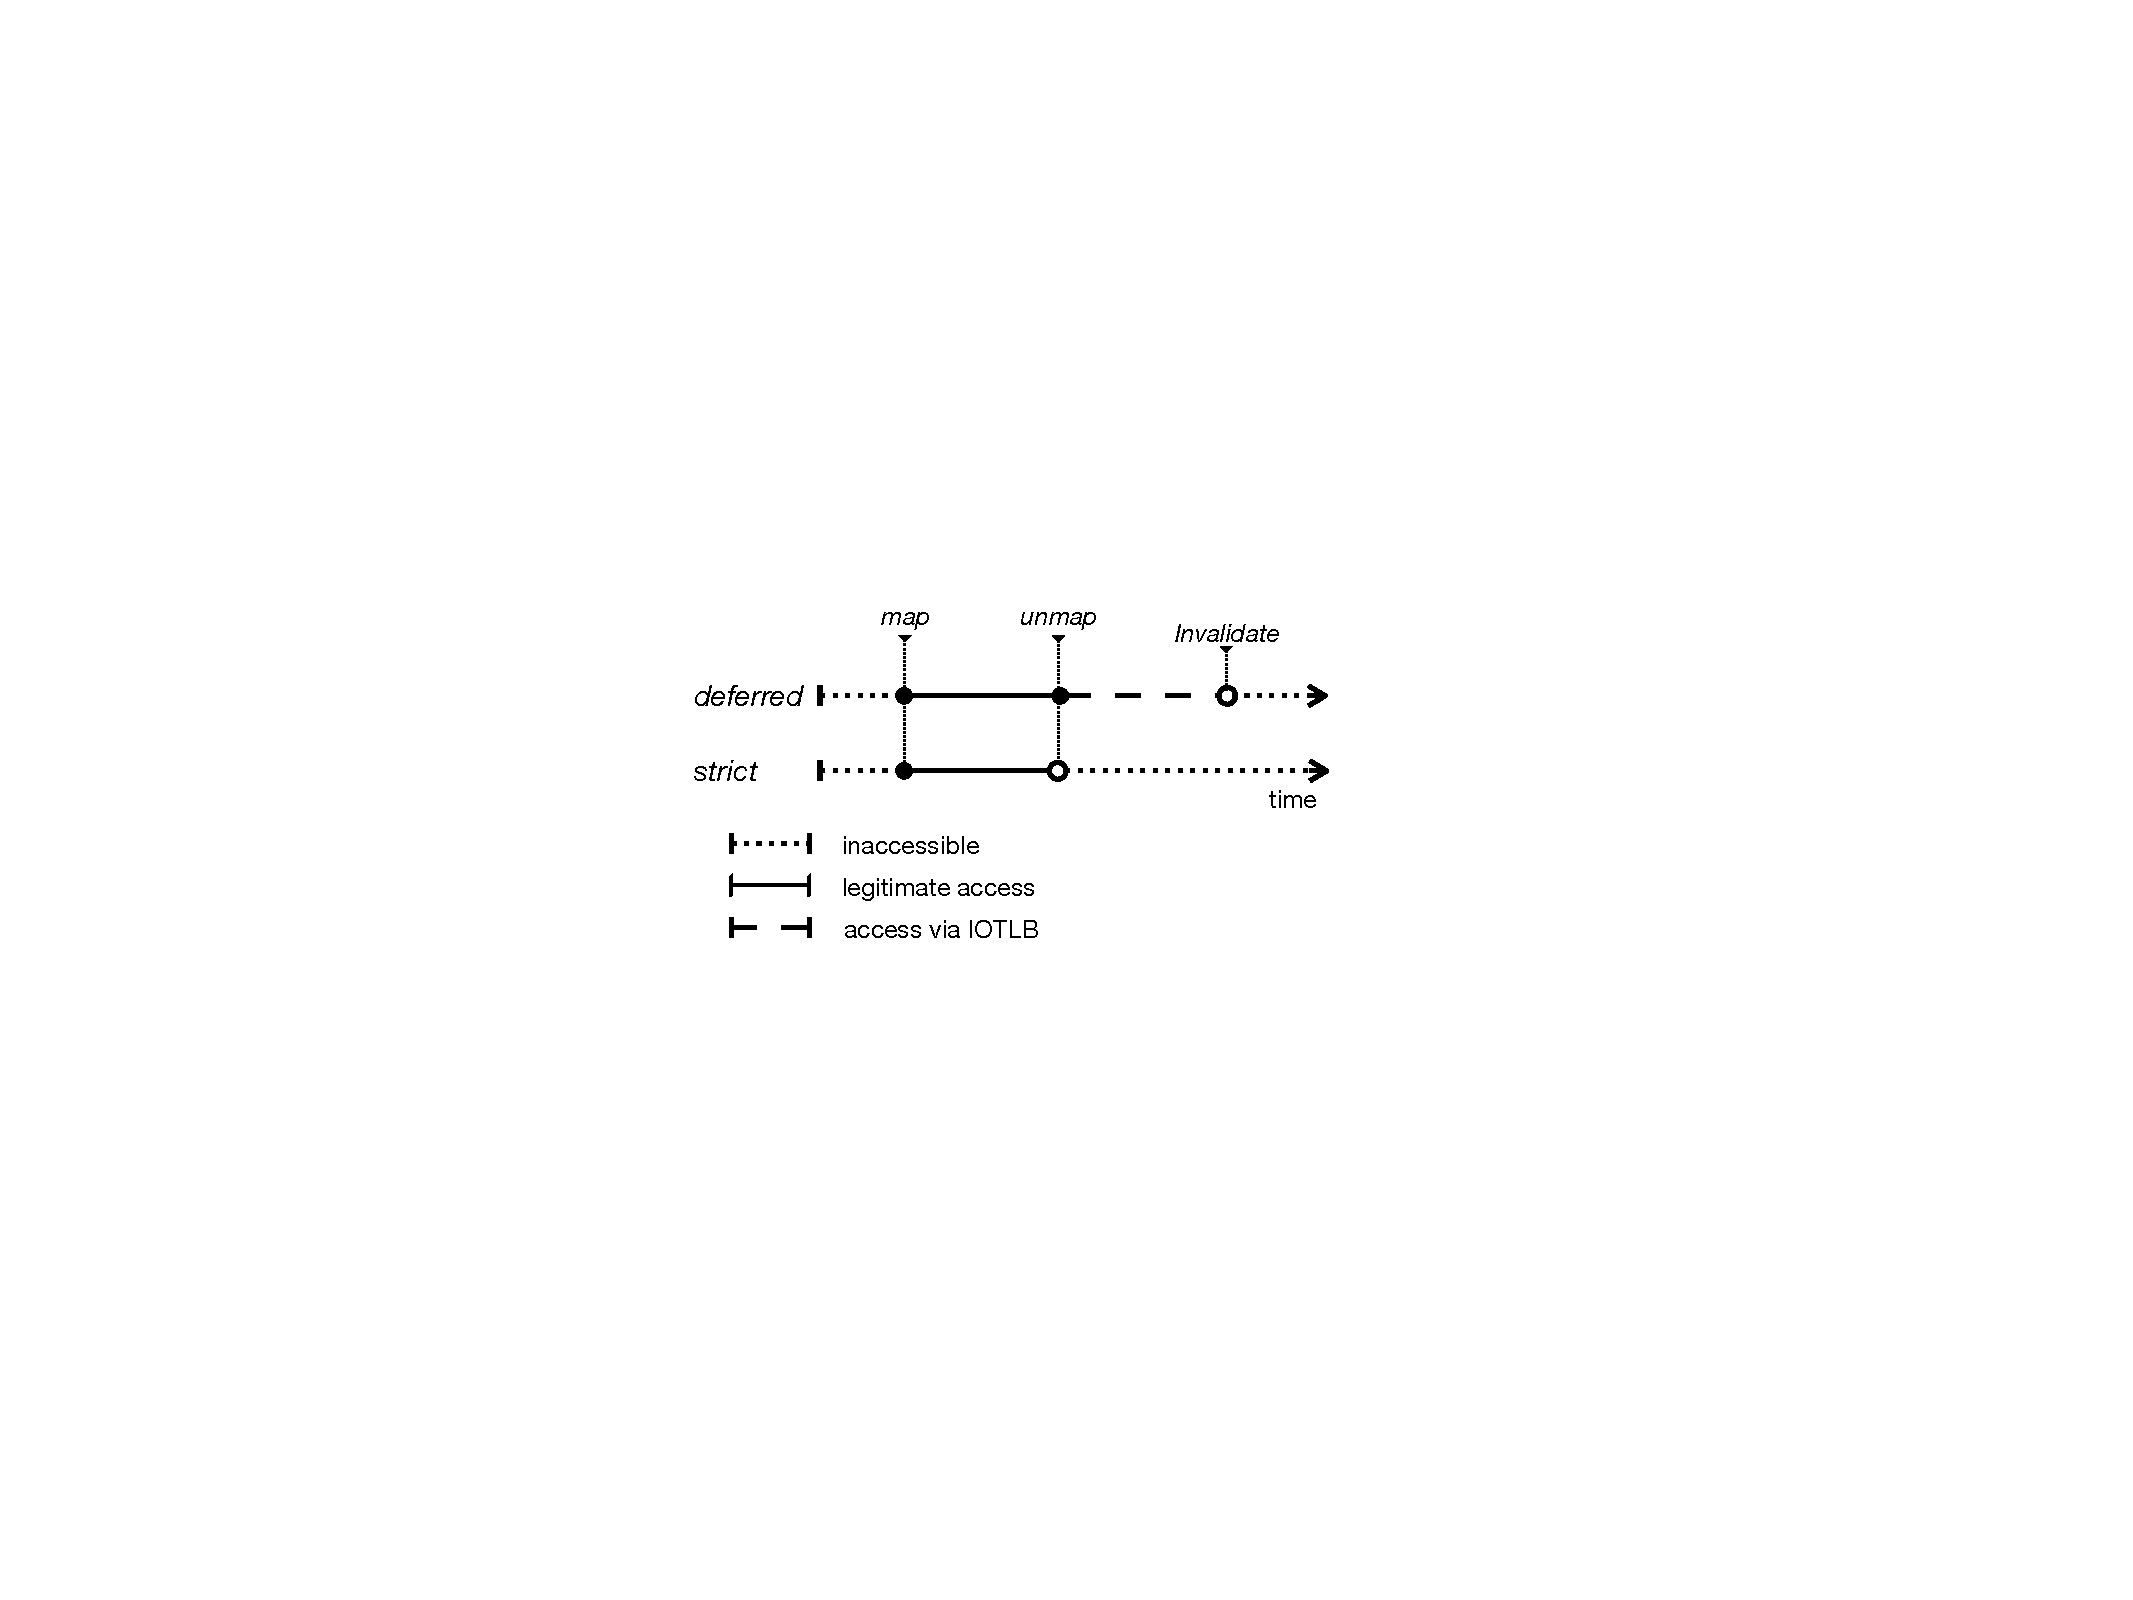
\includegraphics[width=0.75\columnwidth]{figs/strict.pdf}
    \caption{Strict vs. deferred IOTLB invalidation. In \emph{deferred} mode, there is a time window where the data is accessible to the device, but the mapping no longer appears in the page table.}
    \label{fig:deferred}
\end{figure}

\subsubsection{The Time window}\label{sec:shinfo}

\begin{figure}[t]
    \centering
    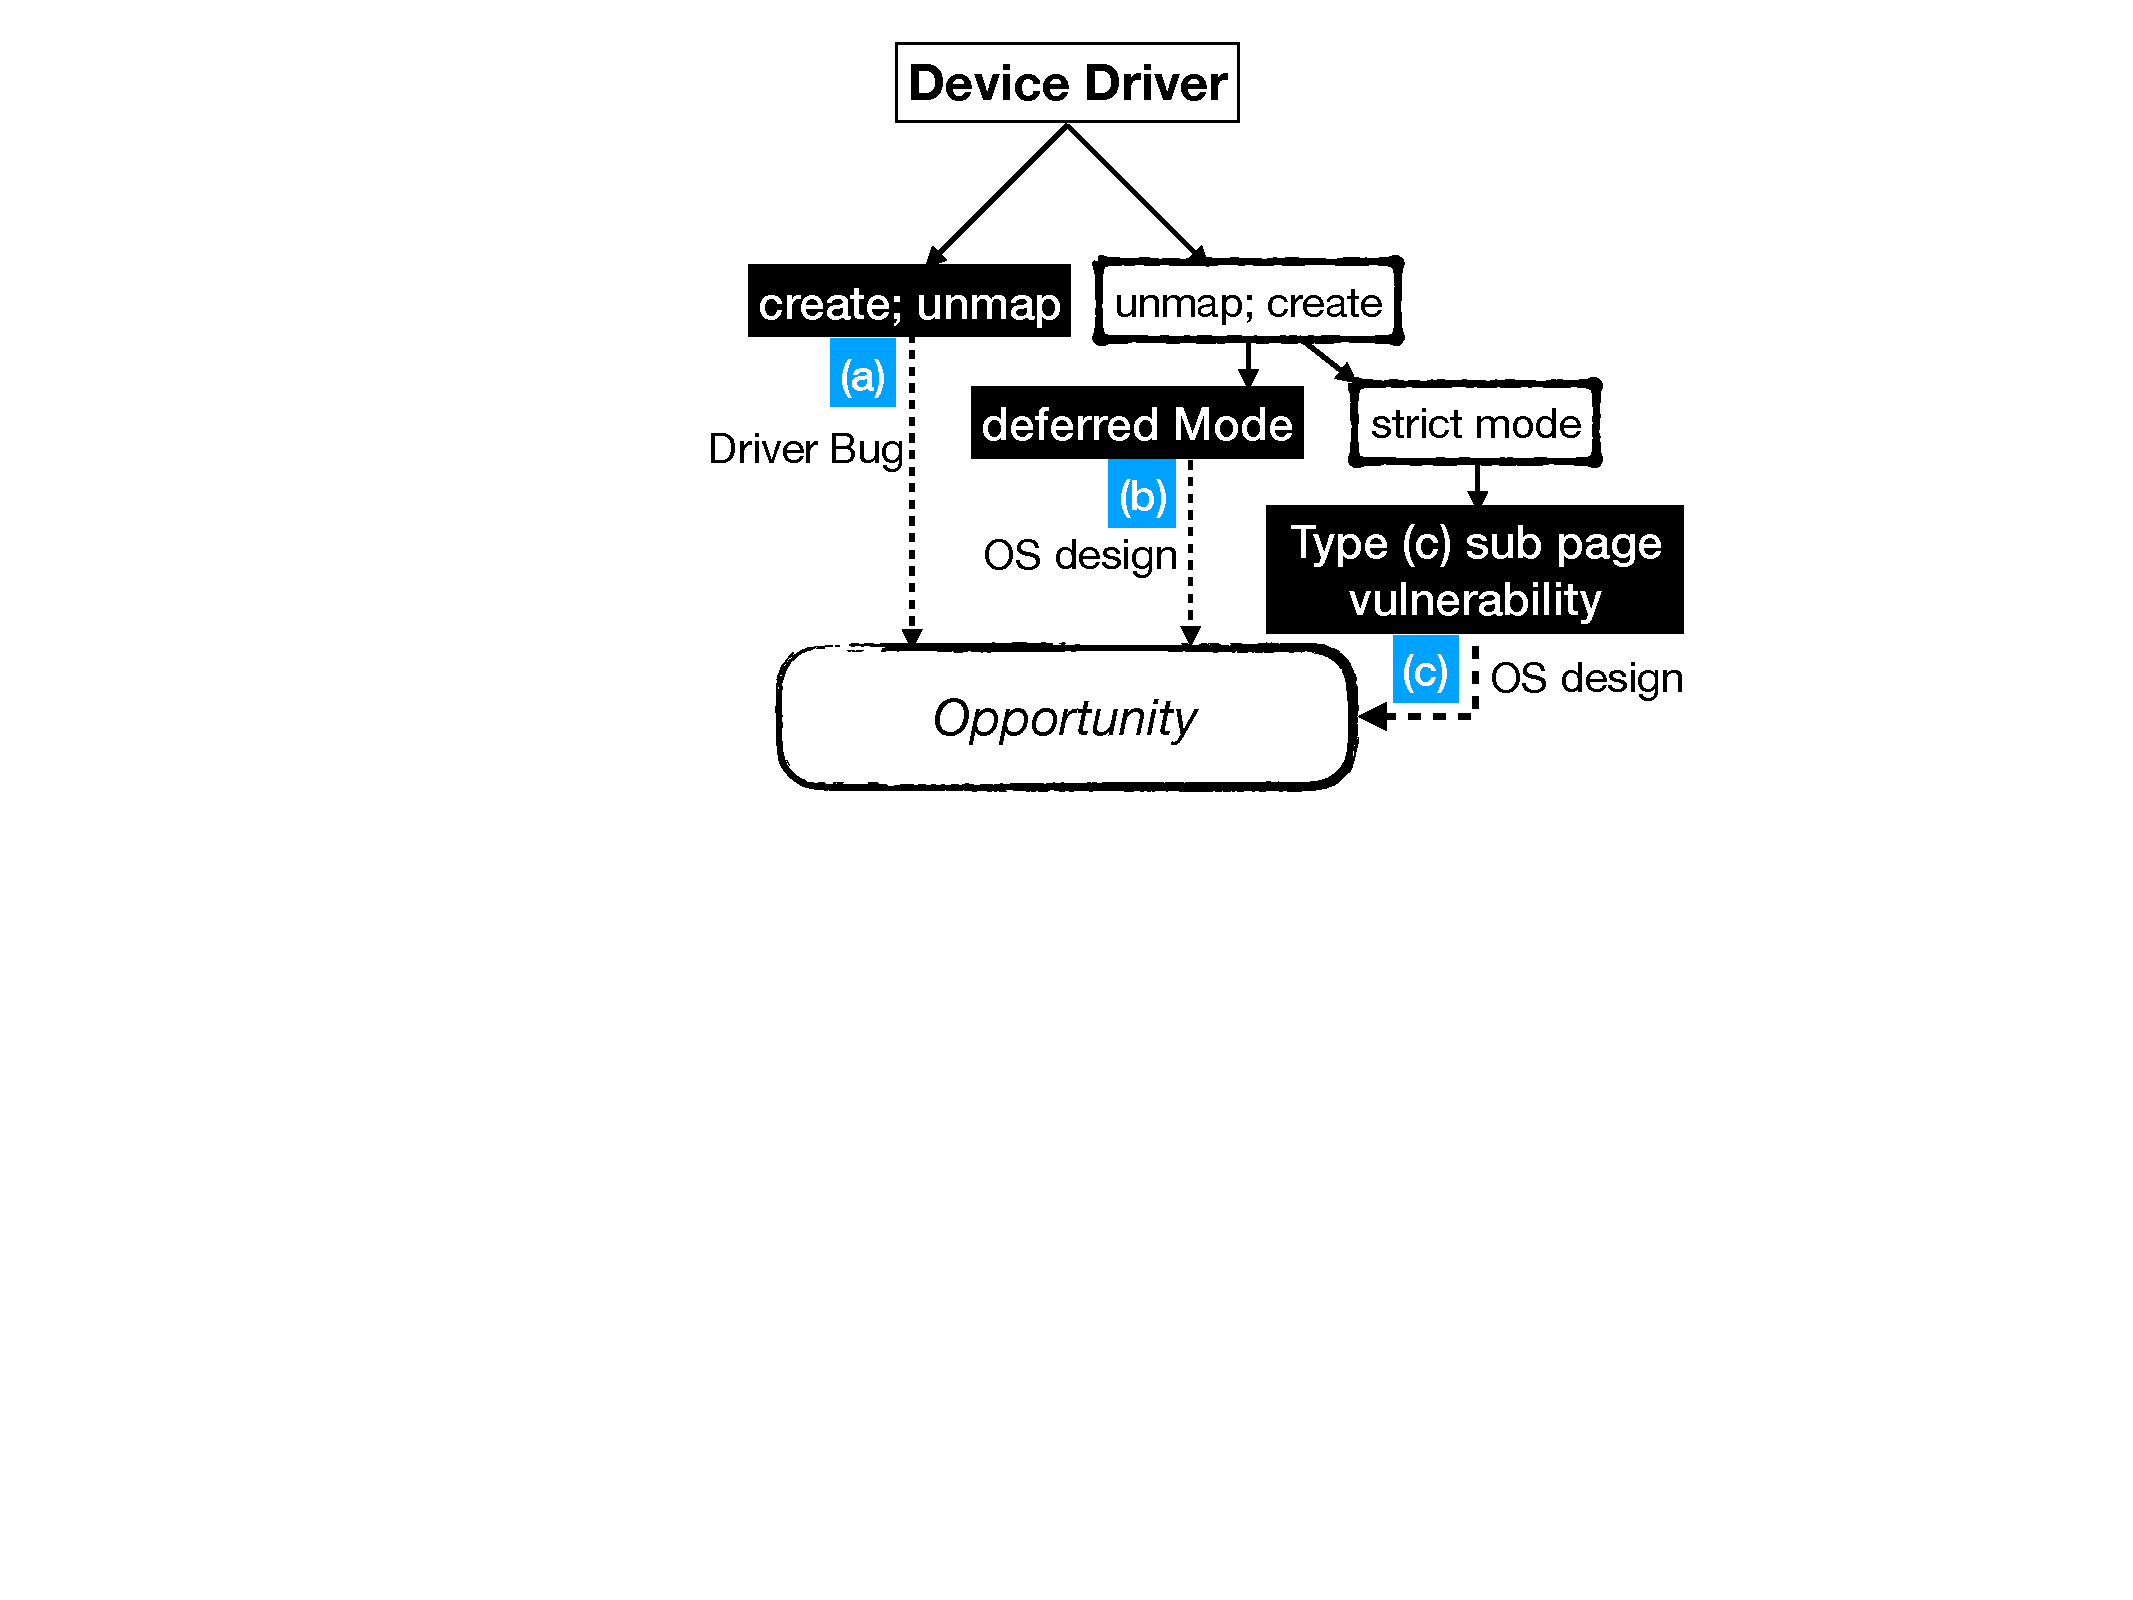
\includegraphics[width=0.75\linewidth]{figs/road_to_op.pdf}
    \caption{Different ways in which the callback pointer in \shinfo can be successfully exploited.}
    %\vspace{-2mm}
    \label{fig:road_to_op}
\end{figure}

%\adam{IMPORTANT POINT: To me, it seemed that the tool sections were about gaining Opportunity.  Why do we now need another section on "Hacking" it? Do the tools not flag the skb-shared-info? If they do, and it's still not enough, how do we know Opportunity exists in the other cases they flag?  Perhaps, the exact goal of the tools and what they find should be described more precisely.}
%\st{We now detail the different ways in which a malicious device can obtain} \oportunity{} (Fig.~\ref{fig:road_to_op}).

%In this section we discuss the Linux network stack where \shinfo is initialized \emph{after} the page was unmapped, thus invalidating the malicious changes.
Upon packet arrival on a receive path, an \shinfo struct is initialised after a packet is received, namely after the DMA operation was completed and potentially the DMA access revoked. In such a case,
a correct use of the DMA API should thwart the attack outlined in Sec.~\ref{sec:shinfo_exploit} (Fig.~\ref{fig:sh_info}). Namely, first unmapping the buffer and only then initializing the \shinfo{} should allow the CPU to undo any malicious changes by the NIC. But, as we demonstrate \textcolor{red}{next}, DMA access is often easily achievable even after the CPU has made its changes. 

We next describe how the time window is attainable via three different paths as illustrated in Fig.~\ref{fig:road_to_op}: 

%\adam{why is this an enumerations?}\SV{added reference to figure 8...}

\begin{enumerate}[label=(\roman*),wide, labelwidth=!, labelindent=0pt]

\item As it turns out, prevalent device drivers (e.g., Intel 40GbE driver, i40e) first create an \skb{} and only then unmap the buffer. This order of execution allows the \emph{device} to undo legitimate changes to \shinfo{} by the CPU. 

\item Nevertheless, even when the order is correct, i.e., the unmapping of the buffer occurs before the creation of the \skb{}, still \shinfo{} is not safe from later modifications. As the default IOMMU mode in Linux is \emph{deferred} protection (Sec.~\ref{sec:deferred}), the unmap order is made irrelevant. That is, even though the unmap function is invoked in the correct order, the device can still corrupt \shinfo{} due to the IOTLB.  

\item In response, a security-conscious admin may change the default setting to \emph{strict} mode, where the IOTLB is flushed on every unmap. However, this both severely degrades networking performance~\cite{MMT16,MSMT18}, and does not alleviate the security threats on the system. Presumably, with \emph{strict} mode enabled, the \iova{} the NIC used to access that \shinfo{} is no longer valid, which initially sounds promising. The problem is that the device, in many cases, still has legitimate WRITE access to the physical page of the \shinfo. The vulnerability stems from the way \data{} is allocated. An RX \skb{} is almost exclusively allocated via an API (e.g., \texttt{netdev\_alloc\_skb}) that creates a type (c) \subpage{} vulnerability (Fig.~\ref{fig:colocation}(c)). The device can use the \iova{} of a co-located buffer to access the \shinfo{} it requires. Particularly, the buffers of the driver RX ring are allocated sequentially, resulting in pairs of successive RX descriptors that map the same page. Obviously, this holds as long as the buffer sizes are smaller than 4 KB. This is a reasonable assumption since the default MTU size is 1500~B. These allocation functions, use a \texttt{page\_frag} mechanism to allocate the \data{} buffers, which in turn contain \shinfo. The \texttt{page\_frag} is an efficient method for allocating small buffers, often used by the Linux network stack (it is used 344 times by network drivers in Linux kernel 5.0). A \texttt{page\_frag} is initialized by allocating a contiguous memory region (usually 32 KB), setting a \textit{va} pointer to the beginning of the region and \texttt{offset} to the end. An allocation request for \texttt{B} bytes subtracts \texttt{B} bytes from the \texttt{offset} pointer and returns the new value of \texttt{offset}. In multi-core environments, the \texttt{page\_frag} uses a different buffer for each CPU and each CPU has a single RX ring. As a result, each RX ring is served by its own (per-CPU) contiguous buffer. (Fig.~\ref{fig:page_frags}). This mechanism for memory allocation results in consecutive \data{} buffers often residing on the same memory page. Due to this type (c) \subpage{} vulnerability, the NIC does not require the invalidated \iova{} to modify the \shinfo. Instead, it can use the \iova{} for the next data buffer.\footnote{Note that the lower 12 bits (the offset on the page) of the \iova{} are identical to the corresponding \kva{} bits.} The device still has write access due to the valid \iova of the next buffer (i.e., the striped area at the end of the page at Fig.~\ref{fig:sh_info}).
\end{enumerate}

\smallskip
\noindent\textbf{\sout{Our setup.}} \sout{The tg3 and mlx5\_core are both vulnerable. The tg3 driver uses the correct unmapping order, but uses the \texttt{netdev\_alloc\_frag} function that results in a type (c) \subpage{} vulnerability. mlx5\_core driver avoids unmapping the RX buffers altogether. \sout{In kernel 5.0, the driver uses a \texttt{page\_pool} mechanism~\cite{page_pool}.} These design choices leave \shinfo{} vulnerable, in both cases, regardless of the IOMMU policy (i.e., \emph{deferred} or \emph{strict}).}


From this point on, we assume that the attacker can always modify the callback pointer. In the next subsections, we demonstrate various compound DMA attacks where an attacker can exploit \textcolor{red}{the} OS design to obtain the kernel virtual address of buffers containing malicious code, completing the trifecta of vulnerabilities.

\subsection{The Ring Flood \Compound{} Attack}\label{sec:ringflod}
A malicious device can generate a poisoned ROP stack in each RX buffer.
However, this is not sufficient to execute a successful code injection attack. 
In particular, the device has all the \iova{} for the RX buffers, but not the \kva{}.
%since the device lacks the corresponding \kva of the RX buffer.

%A malicious device can generate a poisoned ROP stack in each RX buffer. At this point, the device still cannot execute a successful code injection attack since it lacks the corresponding \kva of the RX buffer.
%The device has all the \iova{} for the RX buffers, but not the \kva{}. 

In this attack, we take advantage of the fact that the boot process is \emph{deterministic}. Each reboot, the same set of commands is executed in the same order, initiating the same kernel modules and starting the same processes. While the pages each module receives may vary in a multi-core environment due to timing issues, we do not expect the drift to be too large. 

We evaluate this assumption on our setup running 256 reboots on Ubuntu 18.04 with both kernels 5.0 and 4.15. With the mlx5\_core driver, many PFNs repeat in more than 50\% percent of reboots on kernel 5.0 and more than 95\% on kernel 4.15. The 4.15 driver version allocates much more memory, allocating 64~KB per RX buffer to facilitate the HW LRO feature. We assume an attacker can gain access to an identical setup and identify the most common PFN. Therefore, an adversary with knowledge about the physical setup can deduce a valid \kva{} for one of the RX pages containing a \mabaf. This provides the needed \kva. Thus, the device can execute the attack as shown in Fig.~\ref{fig:sh_info}.\sout{(in this case, the \texttt{destructor\_arg} will most likely indicate a different page, but other than that, the attack scenario is unchanged).}

The success chances of the RingFlood attack increase with the memory footprint of the device driver. The memory footprint, in turn, depends on the NIC capabilities and the number of cores (number of RX rings) on the server. This means that such attacks have higher chances of success on larger machines. 
For example, some NICs have a HW LRO capability\cite{mlx5_lro}, where a NIC can aggregate multiple TCP packets into a single TCP packet, larger than \textcolor{red}{the} MTU (e.g., bnx2x, mlx5\_core). On drivers configured with these options, each RX buffer is 64~KB regardless of MTU. As a result, these drivers have a much larger memory footprint. Mellanox, mlx5\_core driver on kernel 4.15, enables HW LRO and, as a result, allocates 2~GB of memory per physical device port on a 32 core machine. On kernel 5.0, HW LRO is disabled, and the driver allocates 2~KB per entry and thus only uses 64~MB per port.

\begin{figure*}[t]
    \centering
    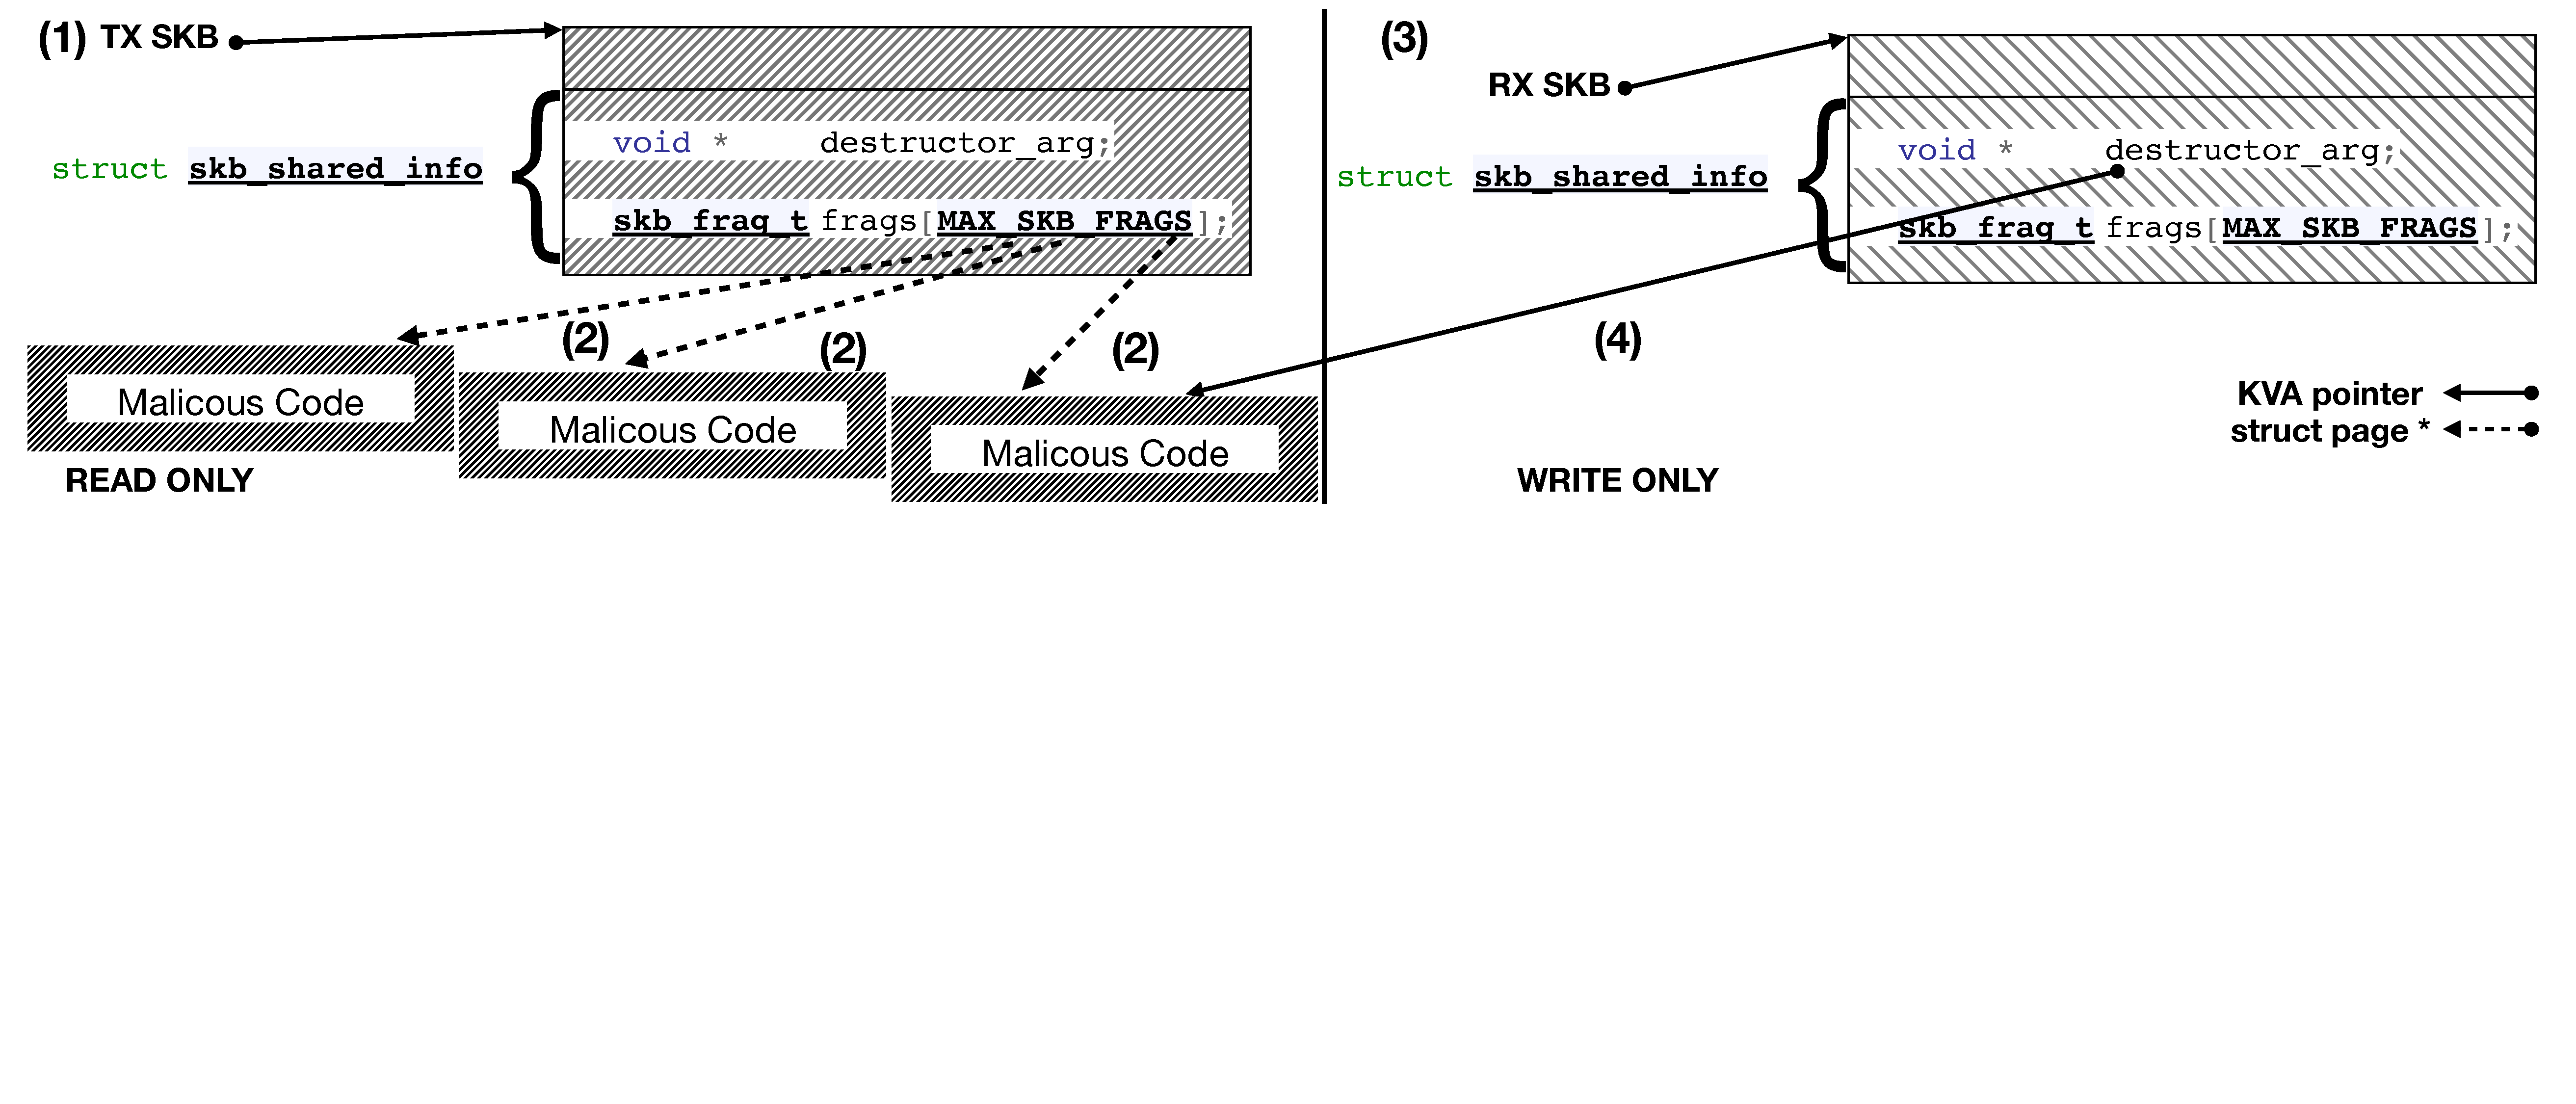
\includegraphics[width=0.8\linewidth]{figs/accomplice.pdf}
    \caption{A TX sk\_buff filled with malicious code provides the \kva for a DMA attack.}
    \label{fig:payload}
\end{figure*}
\subsection{The Poisoned TX \Compound{} Attack}\label{sec:posion}

RingFlood (Sec.~\ref{sec:ringflod}) allows a NIC to execute arbitrary code with high chances of success. However, the prerequisite is sufficient information regarding the server's physical layout and a sufficiently high driver memory footprint. When deducing a valid PFN is not an option (e.g., due to a low memory footprint), another way of acquiring a valid \kva{} is needed.

In this attack, the \kva is acquired by spoofing a malicious transmitted (TX) packet. That is, the attacker gains the needed \kva by \emph{reading} it in the \shinfo of the sent packet. 
%
There are multiple ways in which a malicious NIC device can initiate a TX flow on the server. \sout{We are listing a few examples below}\textcolor{red}{We list a few examples below}:
\begin{enumerate}
    \item Coercing a userspace process into echoing a malicious buffer's contents can be achieved in various ways. For example, a proxy server, a key/value store and, a streaming service.
    \item A cloud VM (e.g., on GCP, AWS, or Azure). A publicly accessible VM may be used to compromise the \emph{host} in the presence of a malicious device.\footnote{Indeed, Google's OpenTitan~\cite{opentitan} exemplifies that cloud providers actively worry about the root of trust for their servers.}
    \item Packet forwarding is enabled on the server.
\end{enumerate}
%\adam{the previous sentence comes out of nowhere. add a sentence explaining the high-level idea of using a user-level process etc. The current sentence about spoofing a malicious packet isn't comprehensible.}\sout{another type of accomplice}\adam{this sounds like willingful co-operation, i.e., attacker-controlled. And that's not the intent}\SV{Rewritten. Better?} 
Since a NIC has READ access to the \shinfo{} of a TX packet, this also provides the NIC with READ access to the \texttt{frags} (Fig.~\ref{fig:payload}) array of \shinfo{}. This array contains \page{} pointers, and thus both leaks kernel pointers that allow the attacker to compromise KASLR and provides the PFNs of specific pages containing the data; pages the device can read.

%\st{Assuming an unprivileged accomplice (witing or unwitting) can open a UDP/TCP socket in user space, this user can transmit a poisoned ROP buffer. For a ROP attack (where the kernel text offset is required), the NIC spoofs an RX packet with the poisoned ROP stack to the accomplice, which in turn is sent back as a TX packet. Once an accomplice sends the packet,}
%Assuming the device can trick a userspace process into echoing a malicious buffer's contents, the device can execute a code injection attack in 4 steps:

Once the content of the malicious buffer is echoed (e.g., via one of the methods mentioned above), the device can execute a code injection attack in 4 steps:  
%
\begin{enumerate}[labelindent=3pt]
    \item The TX \data{} and the fragments are mapped for the NIC to read.
    \item The NIC spoofs an RX packet and delays the completion notification of the TX packets (so that the \mabaf{} will not be released prematurely).
    \item The NIC identifies the poisoned buffer and translates \page{} to \kva{} (Sec.~\ref{sec:kaslr}).
    \item The NIC overwrites \shinfo{} with the \kva{} retrieved during step 3. 
\end{enumerate}

%\st{Tricking a userspace process into echoing a malicious buffer's contents can be archived in various ways. For example, a proxy server, a key/value store, streaming service, etc; another type of accomplice can be a cloud VM (e.g., on GCP, AWS, or Azure). A publicly accessible VM may be used to compromise the \emph{host} in the presence of a malicious device.}
%\footnote{Indeed, Googles OpenTitan~\cite{opentitan} exemplifies that cloud providers actively worry about root of trust for their servers.}

In this scenario, the attacker does not require prior knowledge regarding the physical setup since the echoed buffer provides the \kva.  

%\noindent\textbf{Timing concerns.} 
Note that an attacker will need to delay the TX completion of the echoed buffer to ensure the contents are unchanged until the ROP/JOP attack is executed.
Moreover, a TX completion event that fails to appear in due time will trigger a TX T/O error that flushes all buffers and resets the driver. The T/O is set by the driver, usually to a few seconds, sufficient to complete the attack.
 


%Namely, the only requirement for the success of this attack is an accomplice, witting (e.g., an unprivileged user) or unwitting (e.g., a proxy server) that can open a socket in user-space. For that matter, a socket in user-space of a \emph{guest machine} makes any cloud VM a valid intrusion tool in the presence of a malicious device.

%\smallskip
%\noindent\textbf{User buffer.} An attacker could try storing the \mabaf{} and code in user-space. Such and attempt would fail due to SMEP/SMAP~\cite{smep} as the kernel will not be able to directly execute user-space code.

%\clearpage
%\section{Additional Compound attacks}\label{appx:additional_compound}

\subsection{\textcolor{red}{\textbf{eXpress Data Path}}}\label{sec:xdp}

eXpress Data Path (XDP)~\cite{xdp} provides a way for users to add custom handling to RX buffers with little overhead. Common use cases include DDOS mitigation, forwarding and load balancing. To support the latter, the RX buffers are mapped with BIDIRECTIONAL access to the NIC. 

The tg3 driver does not support XDP. XDP support is usually added to high-speed NICs, such as ConnectX-4 (mlx5\_core). Accordingly, in this attack, we focus on the mlx5\_core driver, which, as mentioned in Sec, \ref{sec:forward}, does not unmap the RX buffers and reuses the pages using the page\_pool mechanism \cite{page_pool}. Subsequently, these pages are never unmapped, and remain accessible to the device for both reading and writing. 

The fact that the NIC has both read and write access to \shinfo, allows the NIC to execute an attack in 4 steps (Fig. \ref{fig:gro_xdp}):
\begin{enumerate}
    \item An RX TCP packet is generated. Then, the \shinfo{} is initialised by the driver and the \texttt{frags} are filled with NULL pointers. Finally, the packet is handed to the next layer.
    
    \item A second RX \skb{} is generated as part of the same TCP stream, initialized and also handed to the next layer.
    
    \item Both packets reach the GRO layer. Then, the second \skb{} is coalesced with the first packet, the \skb{} is freed and the \data{} is added as a \texttt{frag} to the first \skb.
    
    \item The NIC reads the updated \texttt{frag} field and translates the \page{} address to a valid \kva{}. Finally, the device fills the \texttt{destructor\_arg} field, creating a poisoned \skb{} (Fig. \ref{fig:sh_info}).
\end{enumerate}

The difference between this flow and a regular receive flow is the additional read capability the NIC has due to XDP. That is, the last step, where \kva is obtained, is possible only due to the additional READ access.

\smallskip
\noindent\textbf{Remark.} Other drivers that have XDP support, also tend to map RX buffers with BIDIRECTIONAL (e.g., bnxt, i40e, mlx4\_en). Interestingly, the mlx5\_core driver has two modes of operation: (1) linear - where an skb is built around an RX buffer and, (2) non-linear where the driver is filling up the \texttt{frags} of \shinfo, which was never mapped. The former is the default, and the later is actually secure. The non-linear mode is secure because \shinfo{} is \emph{never} accessible to the device. Thus the NIC never gains the oportunity to attack.

\begin{figure*}[t]
    \centering
    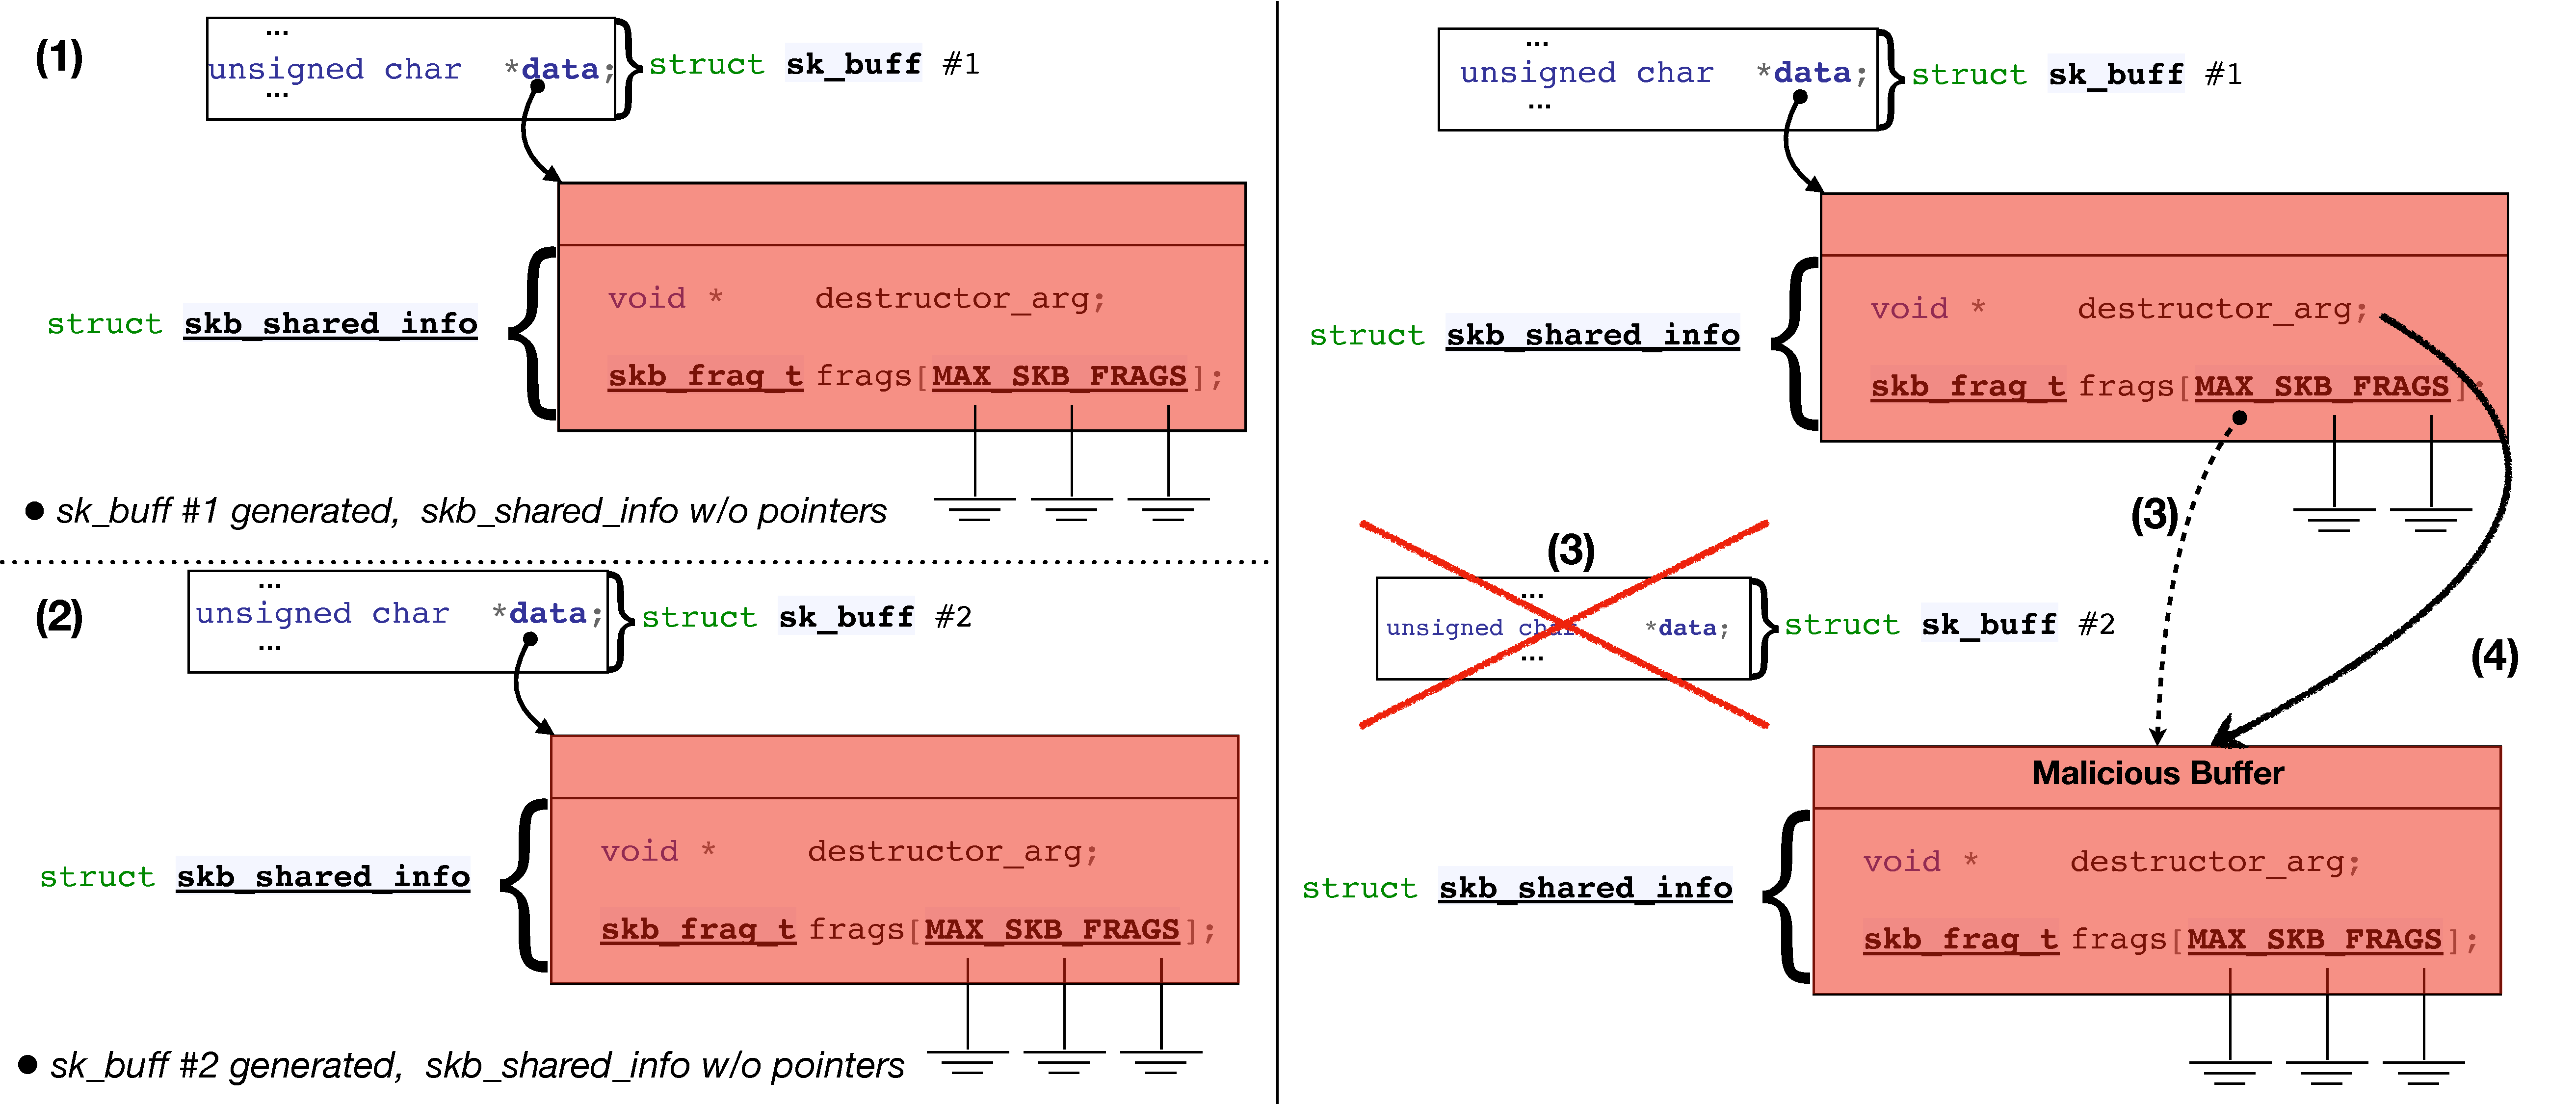
\includegraphics[width=\linewidth]{figs/gro.pdf}
    \caption{An RX \skb{} after GRO provides the \kva{} for a DMA attack.}
    \label{fig:gro_xdp}
\end{figure*}

\subsection{\textcolor{red}{\textbf{Forward Thinking}}}\label{sec:forward}

Packet forwarding is a standard Linux feature that allows a Linux machine to serve as a router or a load balancer. Packet forwarding functionality is usually disabled by default on Linux servers.

When this functionality is enabled, the NIC can independently generate an RX packet to a legitimate destination. This packet will then be forwarded to become a TX packet. However, unlike in the TCP layer that usually creates \skb{} packets with fragments, both the tg3 and the mlx5\_core drivers, usually create a linear \skb{}.

Namely, the drivers do not fill the \texttt{frags}, which the attacker uses to obtain a \kva. Both drivers, use the \\\texttt{napi\_gro\_receive} function to pass the \skb{} to the upper layer (this is the standard for most NIC drivers\footnote{Used by 98 NIC drivers, in Linux 5.0}). 

In this case, the upper layer is the Generic Receive Offload (GRO) layer \cite{gro}. GRO attempts to aggregate multiple TCP segments into a single large packet. Specifically, GRO converts multiple linear \skb{} buffers (belonging to a single TCP stream) into a single \skb{} with multiple fragments. This \skb{} then traverses the Linux network stack and becomes a TX packet. The attacker can use this TX packet as described in the previous attack (Fig. \ref{fig:payload}).

Packet forwarding, also opens up an additional attack option. An attacker might be interested in persistent surveillance rather than overtaking the machine. 

Packet forwarding allows the NIC to inspect arbitrary pages at will. 
Instead of sending a TCP packet and letting the GRO layer fill in the \texttt{frags} information, the NIC can generate a small UDP packet and fill in the \texttt{frags} array with any arbitrary \page{} addresses within the system. This results in the mapping of these pages by the driver, providing READ access to any page in the system to the NIC. Both the mlx5\_core and tg3 drivers map all the frags in \shinfo{} without verifying the actual packet length.

To avoid detection and, more importantly, preserve OS stability, the device must undo the changes to \shinfo{} before creating a TX completion. That is, before letting the CPU know that the packet was sent and its buffer can now be freed. Otherwise, the OS will try freeing the pages, indicated by \shinfo.

\smallskip
\noindent\textbf{Remark.} Having an accomplice in the form of an unprivileged user provides an additional vectors of attack. In addition to running ROP attacks, the NIC can also leak the content of arbitrary memory pages to the user. Assuming that the NIC has WRITE access to \shinfo{} after it has been sent up the network stack (for example, in case of deferred protection or when page\_pool is used, Sec. \ref{sec:xdp}), the NIC can modify the \page{} address in the \texttt{frag} entries, letting the Linux network stack copy the context of arbitrary memory pages to an unprivileged user. A likely side effect of this attack is memory corruption and Kernel panic, so caution is advised. The reason being, that the \texttt{skb\_free} function attempts to free pages never owned by the network stack.




